%************************************************
\chapter{Reference Implementation}\label{ch:implementation}
%************************************************

\autoref{ch:flexibleeventsubscription} has presented a concept that involves the model layer, the process engine and the event engine.
It enables flexible event subscription in BPMN to overcome the issues revealed in \autoref{ch:problemstatement}.
The model extension is described in \autoref{ch:bpmnx}, and allows to create BPMN models that contain all information necessary to to issue event subscriptions for the employed event elements.
To evaluate the results we enhance the business process engine Camunda and the event processing platform UNICORN following the procedures described in \autoref{ch:extendedprocessengine} and \autoref{ch:bufferedcep} respectively.
Camunda is extended by providing a Process Engine Plugin (\autoref{ch:implcamunda}), Unicorn by adapting the source code (\autoref{ch:implunicorn}).
\autoref{fig:architecture-camunda-unicorn} shows an overview of the applied architecture with added and modified elements highlighted in gray.

\begin{figure}[]
	\myfloatalign
	{\hspace*{-2.3cm}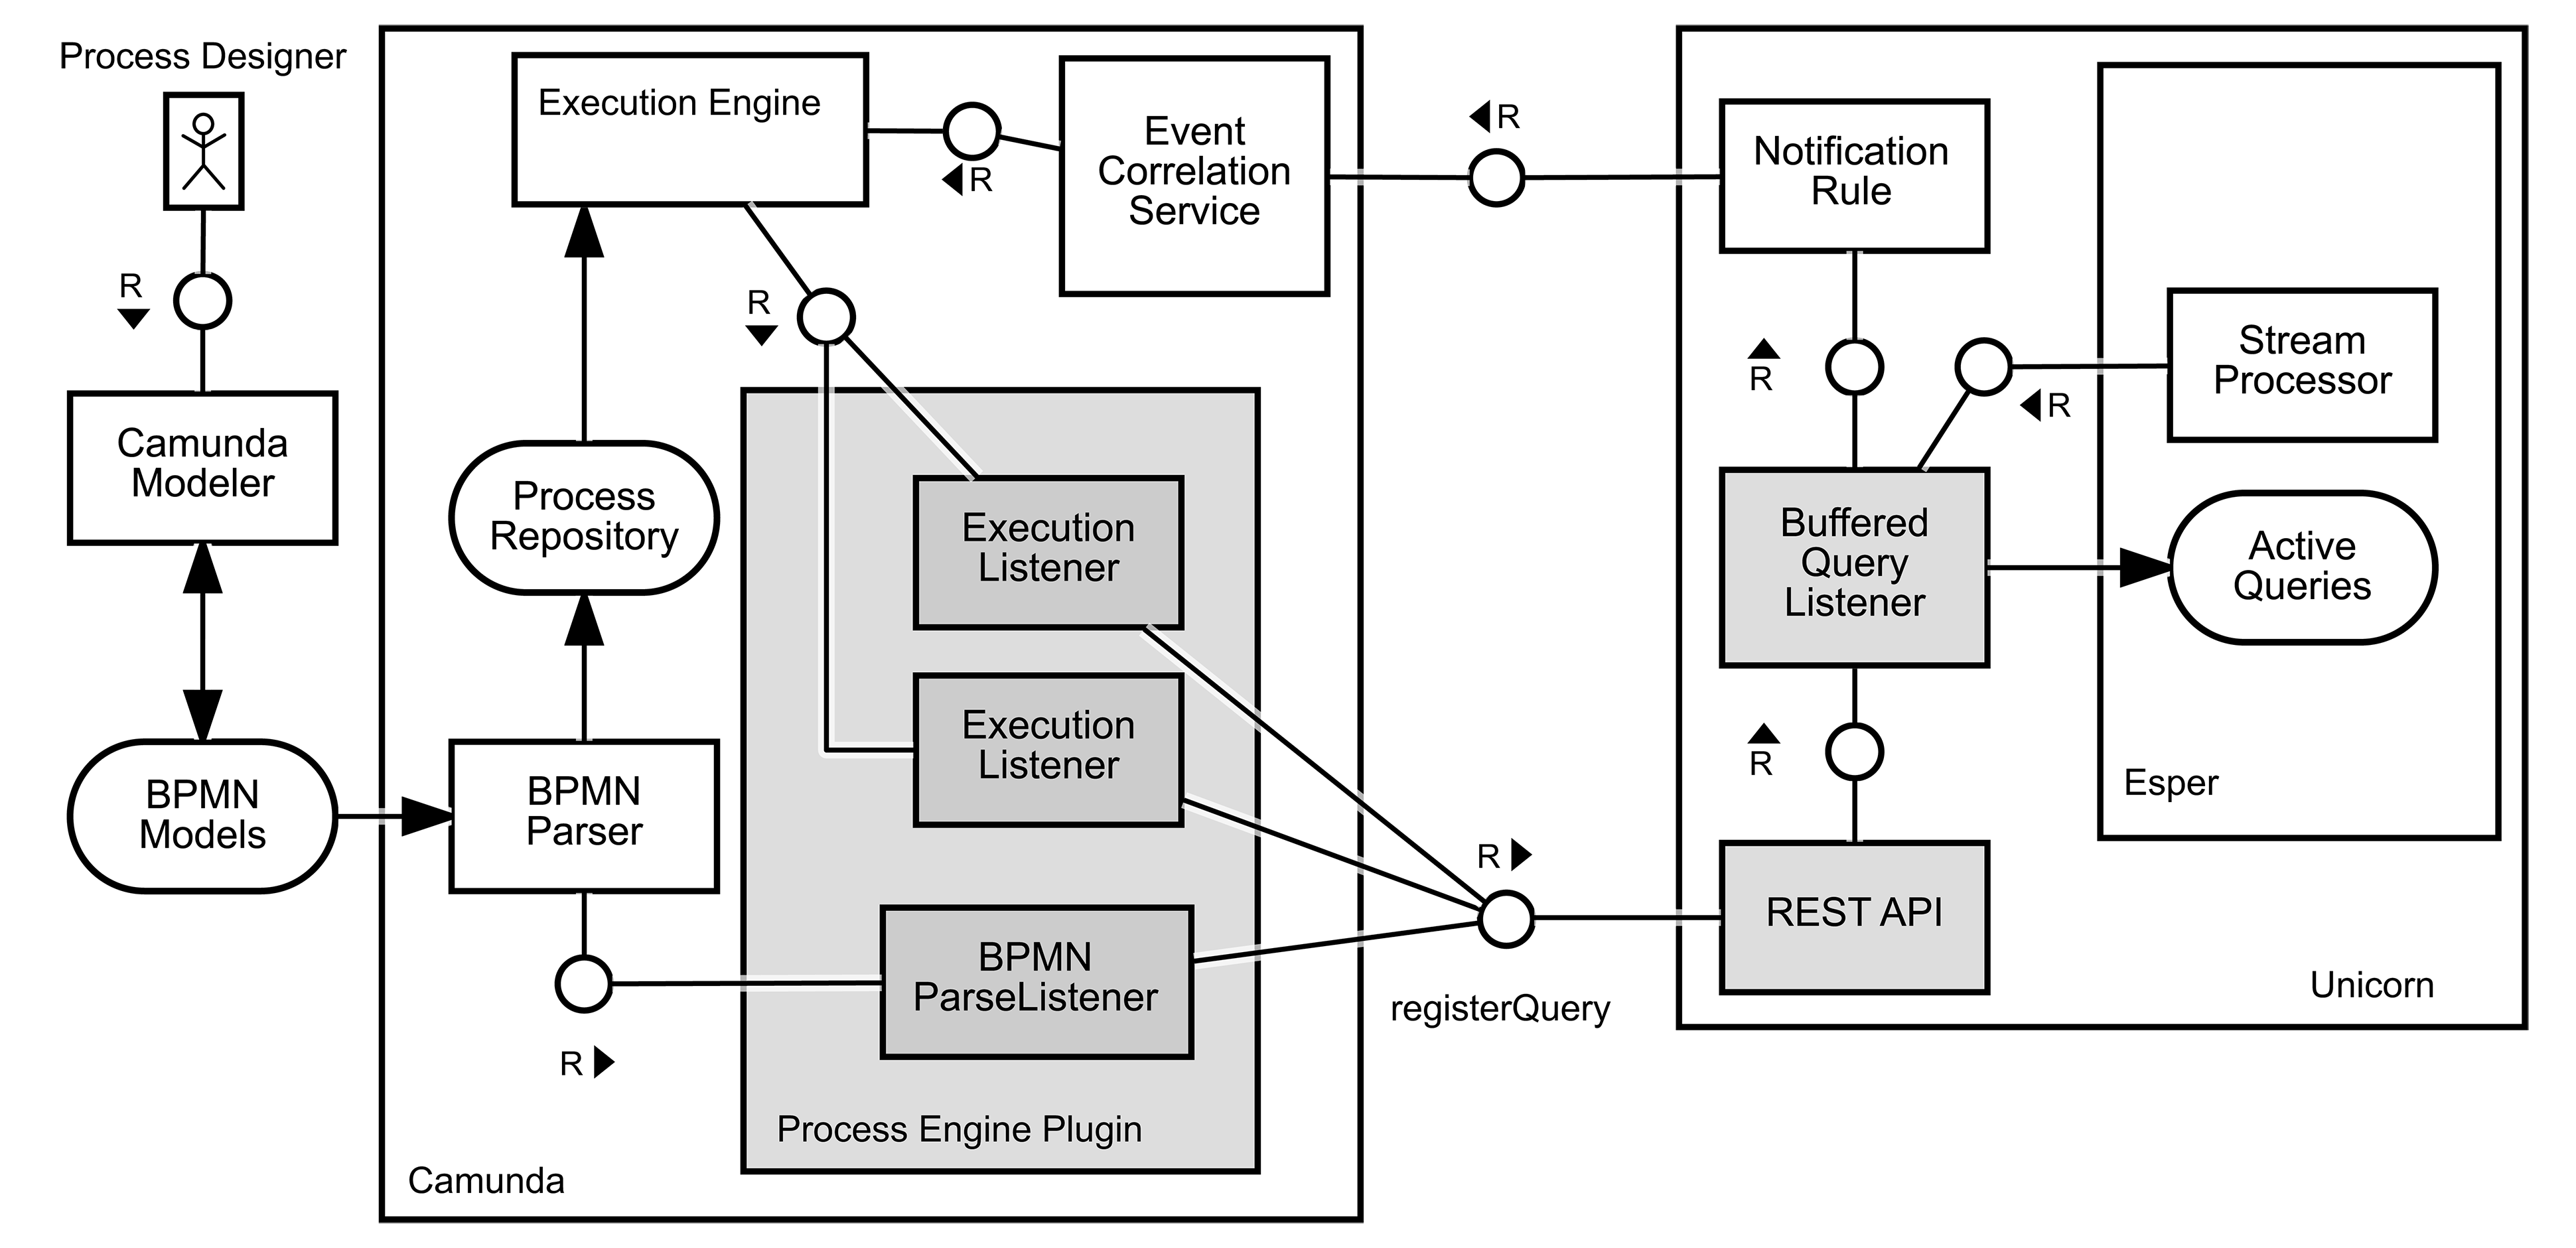
\includegraphics[width=1.3\linewidth]{chapters/implementation/flexible-evt-subscr-camunda-unicorn.png}}
	\caption{Architecture for flexible event subscription in Camunda and Unicorn}
	\label{fig:architecture-camunda-unicorn}
\end{figure}


\section{Extending the Event Processing Platform Unicorn}\label{ch:implunicorn}
\textit{UNICORN} is an event engine developed for academic purposes at the Business Process Technology chair of the Hasso-Plattner-Institute, Potsdam \cite{unicornhome, baumgrass2015get}.
%It focuses on event processing for \acs{BPM}
It has been developed in the course of the EU \textit{GET project} \cite{getservicehome}, which investigates options to increase efficiency in logistics.
Unicorn is based on the Esper \cite{esperhome}, an open source component for complex event processing available in Java.
Esper can be integrated into custom applications using its feature-rich Java API and will provide stream processing capabilities including an own \acf{EPL}.
Unicorn integrates Esper and adds a web-based user-interface, a REST API, a persistent data-store for events and a number of features specifically related to BPM.
The latest version of Unicorn uses Esper $5.3.0$, therefor all future considerations are made based on the documentation of that version.

\autoref{ch:bufferedcep} considers three architectural options to provide buffered event handling capabilities.
It has been decided to extend the event engine in this scenario for several reasons.
Firstly, the performance and operation of the process engine shall not be jeopardized (see shortcoming \textit{S3} in \autoref{ch:ass:discussion}). Event Processing features potentially require a lot of performance to handle a large number of requests in a short amount of time.
By implementing the event Buffering module loosely coupled to the Process Engine, we ensure that its performance is not influenced.
Implementing a separate middleware was avoided in the course of this work, to keep the architecture easy and concise to describe.
Unicorn is an academic prototype in constant development and therefor predestined to be directly extended for this kind of use-case.
Moreover, the chosen architecture promises performance advantages thanks to running the event buffering in the same \acs{JVM} as Esper.


\subsection{Event Buffering}
To allow the delayed delivery of events, buffering functionality is added to Unicorn.
Whereas, originally, events that match a certain query in esper are directly forwarded to the notification-recipients, they will instead be held in a buffer until requested by recipient. 
If a recipient is already subscribed, than the behavior will be equivalent to the original scenario, because the event will be delivered instantly.

\paragraph{Engine-specific Implementation Options}
When investigating the options for implementing event buffers in UNICORN, solutions that are specific to the event processing platform were considered.
Notably, the concept of a \textit{Window} in event processing languages is very much comparable with a buffer as described in this work. Windows hold a variable number of events in memory according to specified window properties. That way, windows can act like size- or time-oriented buffers and allow access to older events whenever a new event occurs.
\textit{Named Windows} in Esper allow to create global data windows that can be modified and read from multiple statements. Similar functionality is provided by \textit{Tables}, which follow a relational approach by primary key.
\footnote{see \textit{Chapter 6. EPL Reference: Named Windows And Tables}, \url{http://www.espertech.com/esper/release-5.3.0/esper-reference/html/nwtable.html}, accessed 2017-08-12}

If a query window is connected with the Esper-specific \textit{Output Clause}, it is possible to delay query output with timing constraints or trigger it on the change of a global variable.
\footnote{see \textit{Chapter 5. EPL Reference: Clauses}, \url{http://www.espertech.com/esper/release-5.3.0/esper-reference/html/epl\_clauses.html}, accessed 2017-08-12}
When putting together these features, an event buffer could be implemented as follows: The call \textit{registerQuery} instantiates the window. If the \textit{Consume}-policy is used, we use a named window that we share among queries and delete from after receiving the event. 
At \textit{subscribe}, a notification-recipient is added to a query and output is triggered by causing a variable change in Esper. \textit{Unsubscribe} and \textit{removeQuery} remove a notification-recipient and de-register the query respectively.

A major drawback of this approach is, that the event queries have to be adopted to use the specific features which makes additional knowledge necessary when designing the processes.
Alternatively, the original queries submitted by the process engine can be transformed before registering them in Unicorn, for example by encapsulating them in a sub-query. That way they make use of the mentioned features, but certain expressions will not be possible anymore due to limitations of the Esper EPL with regards to sub-queries.

Apart from this approach, it is worth noting that Unicorn offers a persistent storage of historic events, which can theoretically be used to implement the buffering functionality.
However it would be necessary to abuse the relational approach to implement a persistent stream buffer on top of the SQL database, which is not desirable.

\paragraph{The Generic Buffering Solution}
The investigation of engine-specific solutions did not bring up an optimal solution to implement an event buffer with existing mechanisms.
Furthermore, this reference implementation should not be entirely limited on one specific event engine.
For that reason a new generic buffering module has been implemented within Unicorn. 
%A \acs{UML} class diagram is provided in \autoref{}.
%\missingfigure{UML class diagram of: BufferedLiveQueryListener extends LiveQueryListener, BufferManager (list<EventBuffer> | createBuffer, updatebuffer, deleteBuffer) implements runnable, EventBuffer (Policies | update, maintain, retrieve), Constants}

The module is built around the \textit{EventBuffer}-class. Objects of the class are managed by the \textit{BufferManager} and represent a single buffer entity, holding events of one query. Esper provides the query output as an object of type \textit{EventBean}, which is stored in a list in \textit{EventBuffer}.
The buffer behaves according to the value of its policies, which influence the length of the list, the order in that items are retrieved from the buffer and the consumption behavior.
The lifetime-policy, which requires that events are deleted from the buffer after a certain time, is ensured by a maintenance-thread that runs from the BufferManager class and iterates over all EventBuffer objects in a specified time interval. The default value is 5~seconds.

Unicorn uses the \textit{LiveQueryListener} to react on new event-occurrences. It implements the Esper \textit{UpdateListener}-interface and is registered in Esper as callback-function for a new query. Whenever an event matches that query, the object of \textit{LiveQueryListener} is notified.
Originally, the QueryListener notifies all notification-recipients that are known for that query and then drops the event.
For the event buffering, a new class \textit{BufferedLiveQueryListener} is created which extends the behavior of the standard query listener. Instead of only notifying all recipients, it also updates the associated buffer instance with the latest query output.
The provided implementation serves for demonstration and reference purposes. It is not optimized for performance, for example in the case of overlapping data between buffers. Considering an event subscription issued on process instantiation, multiple \textit{EventBuffer} instances will essentially store the same data, if multiple instances of the process are started at the same time or with minimal difference.

The presented buffering module supports the temporary storage of query results as demanded by the BPMN extension. After query creation, matching events can be stored in a buffer to be retrieved when necessary.
All buffer policies described in \autoref{ch:bpmnx:bufferpolicies} have been implemented.
The following section explains how the \acs{REST}~\acs{API} of Unicorn is extended to make use of the buffering module.

\subsection{REST API Extension}\label{ch:impl:unicorn-api}
Unicorn offers a webservice that allows users to interact with the event processing engine via the \ac{HTTP}.
The restful API comprises the most basic functionality, query registration, query deletion and obtaining query strings by the subscription identifier.
An interaction generally works as follows: The user executes a POST to \textit{<platform>/EventQuery/REST}, providing an event query and information about the desired notification-recipient~(\textit{notification path}). Unicorn registers the query in Esper and returns a unique identifier to the user.
Whenever an event matches the query, the platform sends a notification to the specified recipient. a DELETE call to \textit{<platform>/EventQuery/REST/\{eventQueryUuid\}} triggers the removal of the query.

In accordance with the API requirements introduced in \autoref{ch:bufferedcep}, additional functionality has been added to the Unicorn Webservice.
The methods were added under a new path \textit{/BufferedEventQuery} to make sure that the existing features remain. They are as follows:

\begin{description}
	\item[register query]
		POST to /BufferedEventQuery, returns queryId\newline
		Payload: JSON~(eventQuery[, bufferPolicies]) with\newline bufferPolicies:(lifetime, consumption, size, order)
		
		Description: The provided eventQuery is registered in Esper using a BufferedLiveQueryListener. The BufferManager is used to instantiate a new EventBuffer object. The payload JSON object bufferPolicies is optional, and will be passed to the EventBuffer if available. Otherwise, the system falls back to the default values~(\autoref{tab:bpmn-extension}).
		A unique identifier of that query and associated buffer is returned.
	\item[subscribe]
		POST to /BufferedEventQuery/\{queryId\}\newline
		returns subscriptionId\newline
		Payload: JSON~(notificationPath) with\newline notificationPath:(notificationAddress, processInstanceId, messageName)
		
		Description: An new subscription is added to the selected query, so that a notification is issued based on the current buffer content and whenever an event matches the query.
		The notification-path is specified including the id of the target process instance and the message name. This enables Camunda to automatically correlate the issued notification to the right process execution and message.
	\item[unsubscribe]
		DELETE to /BufferedEventQuery/\{queryId\}/\{subscriptionId\}\newline
		Description: Remove the specified subscription from the list of subscriptions of the selected query.
	\item[remove query]
		DELETE to /BufferedEventQuery/\{queryId\}\newline
		Description: Remove the query and the associated buffer from the system.
\end{description}


%\paragraph{Enabling Event Correlation in Camunda}
Using instances of \textit{NotificationRule}, Unicorn sends notifications to the recipients~(see~\autoref{fig:architecture-camunda-unicorn}). In our scenario, the messages must be sent to Camunda, more specifically to a specific process instance within the engine.
The \textit{Event Correlation Service} within Camunda is responsible for relating incoming message events to process instances. One way to enforce the correlation is by inserting the process instance identifier and the message name inside the message.
For that reason, message name and process instance id must be provided when adding a subscription in the event engine. 
Unicorn has been adopted to send notifications to Camunda including the required correlation information. A sample notification for a eurotunnel delay event is shown in~\autoref{lst:unicorn-json-notification}.
%https://docs.camunda.org/manual/7.7/reference/rest/message/post-message/

\begin{lstlisting}[caption={Example of a JSON notification sent by UNICORN},label=lst:unicorn-json-notification]
{
  "messageName":"eurotunnelDelay",
  "processInstanceId":"274a876f-aed7-4a1a-916b-e85a0c2416f7",
  "processVariables": { 
    "eurotunnelDelay":{"value":"60", "type":"Integer"}
  }
}
\end{lstlisting}

After implementing the necessary extensions to the event engine, it is the task of the process engine to connect the extended process model to the buffered event handling API.
The adaptations to the process engine are presented in the following section.

\section{Event Subscription Handling in Camunda}\label{ch:implcamunda}
%\todo[inline]{In Camunda, data objects can only be used for documentation purposes. The engine ignores them, so there is no way to set a value.}

Through the BPMN extension for flexible event subscription, the information necessary to register event queries in a CEP platform can be made available in process models.
\autoref{ch:extendedprocessengine} outlines how the business process engine must be adapted to execute the operations for subscription handling.
Camunda is an open-source business process engine with support for the latest version of the BPMN and used to exemplify the modification process. Further information about Camunda is provided in \autoref{ch:bg:bpms}.

\autoref{fig:architecture-camunda-unicorn} depicts a simplified architecure of Camunda, highlighting modifications in gray.
Our workflow for flexible event subscription mainly involves the core components, execution engine, model repository, correlation service and the Camunda modeler.

\subsection{Process Engine Plugin and ExecutionListeners}
Being a community-driven open-source project, the Camunda project offers numerous options for customizing and extending its behavior.
A core concept to trigger the execution of custom code during a process execution are \textit{ExecutionListeners}.
They can be incorporated in BPMN models using the properties window of the Camunda Modeler as demonstrated in \autoref{ch:assessment}. In that case they have a textual representation in the model file, a specification can be found in the product documentation
\footnote{\textit{Camunda BPMN Extension Elements}, \url{https://docs.camunda.org/manual/7.7/reference/bpmn20/custom-extensions/extension-elements/\#executionlistener}, accessed 2017-08-10}.

However, one of the main goals of this thesis is to provide an alternative solution to explicitly modeling the subscription, unless an explicit subscription task shall be used). Thus the additional necessity attach execution listeners to BPMN elements shall be avoided.
Instead, subscriptions shall be managed automatically by the process engine solely based on the subscription definition provided in the extended message element.
To achieve this kind of behavior, Camunda offers the concept of a \ac{PEP} to intercept significant engine operations and introduce custom code. 
By this means, execution listeners can be added programatically.
The plugin is a separate software module that implements the interface \textit{ProcessEnginePlugin}
\footnote{\textit{Process Engine Plugins}, \url{https://docs.camunda.org/manual/7.7/user-guide/process-engine/process-engine-plugins/} accessed 2017-08-10}.
It is activated by adding a \textit{plugin} entry in the process engine configuration.

\cite{mandal:2017} and \cite{Pufahl2017} have chosen to directly adapt the source code of camunda. More precisely, they propose to modify the \textit{Behavior} class of the Camunda core to execute additional code when a BPMN element starts executing.
In this work, we implement a Process Engine Plugin as it allows a clearer, more understandable approach to adopting the execution behavior. 
That holds especially when it is only necessary to execute additional operations and not modify or delete existing code.
Moreover, the PEP facilitates the re-usability across environments and different versions of Camunda.

% interface def https://docs.camunda.org/javadoc/camunda-bpm-platform/7.7/?org/camunda/bpm/engine/impl/cfg/ProcessEnginePlugin.html
% peps https://docs.camunda.org/manual/7.7/user-guide/process-engine/process-engine-plugins/


%from \autoref{ch:bpmnx:basic}
%\todo[inline]{that means that in the implementation we need additional configuration values -> implementation chapter}
%- PEP config properties: cep url

\subsection{Managing Event Subscriptions at Runtime}
The Process Engine Plugin enables us to execute custom JAVA code at predefined points during engine execution.
An entry point to the modification of the execution behavior is provided through the implementation of the \textit{ProcessEnginePlugin} interface. It allows to intercept \textit{preInit}, \textit{postInit} and \textit{postProcessEngineBuild}, that means at three different points during the engine bootstrapping.
We chose to provide a custom implementation for the \textit{preInit} method, which has an object of \textit{ProcessEngineConfigurationImpl} as parameter.
With the engine configuration available, a plethora of custom handlers, validators and listeners can be registered\footnote{Some arbitrary examples are pre-/post-deployers, event-handlers, post-variable-serializers, command-interceptors. Full list available from: \url{https://docs.camunda.org/javadoc/camunda-bpm-platform/7.7/org/camunda/bpm/engine/impl/cfg/ProcessEngineConfigurationImpl.html}, accessed 2017-08-11}.

We implement a \textit{BPMNParseListener} that is to be executed after a BPMN element finished parsing~(\textit{customPostBPMNParseListeners}).
The BPMNParseListener interface allows us to react to the parsing of single elements based on their type by making a separate method for every BPMN element available.
A helpful example for using that listener is also provided on GitHub\footnote{GitHub, \textit{camunda-bpm-examples/process-engine-plugin/bpmn-parse-listener}, \url{https://github.com/camunda/camunda-bpm-examples/tree/master/process-engine-plugin/bpmn-parse-listener}, accessed 2017-08-11}.
The BPMN extension affects the intermediate and boundary message catch event, the receive task, the explicit subscription task and can also be used to specify subscription information for a message start event.
It was attempted to utilize the separate methods of every element, but it is not possible to access the subscription information in the associated message elements from that point. Apart from the provided method arguments, the engine's \textit{RepositoryService} can normally be used to view model information, but only after the deployment was finished.  
To overcome this limitation, we implement the method \textit{parseRootElement}, to which a representation of the root element \textit{bpmn:definitions} is passed, including all message and extension elements. 
Before the content of this method is described, two more aspects need to be introduced, the \textit{SubscriptionEngine} and the \textit{ExecutionListeners}. An excerpt of the related UML class diagramm is depicted in \autoref{fig:camunda-ext-uml}.

\begin{figure}[]
	\myfloatalign
	{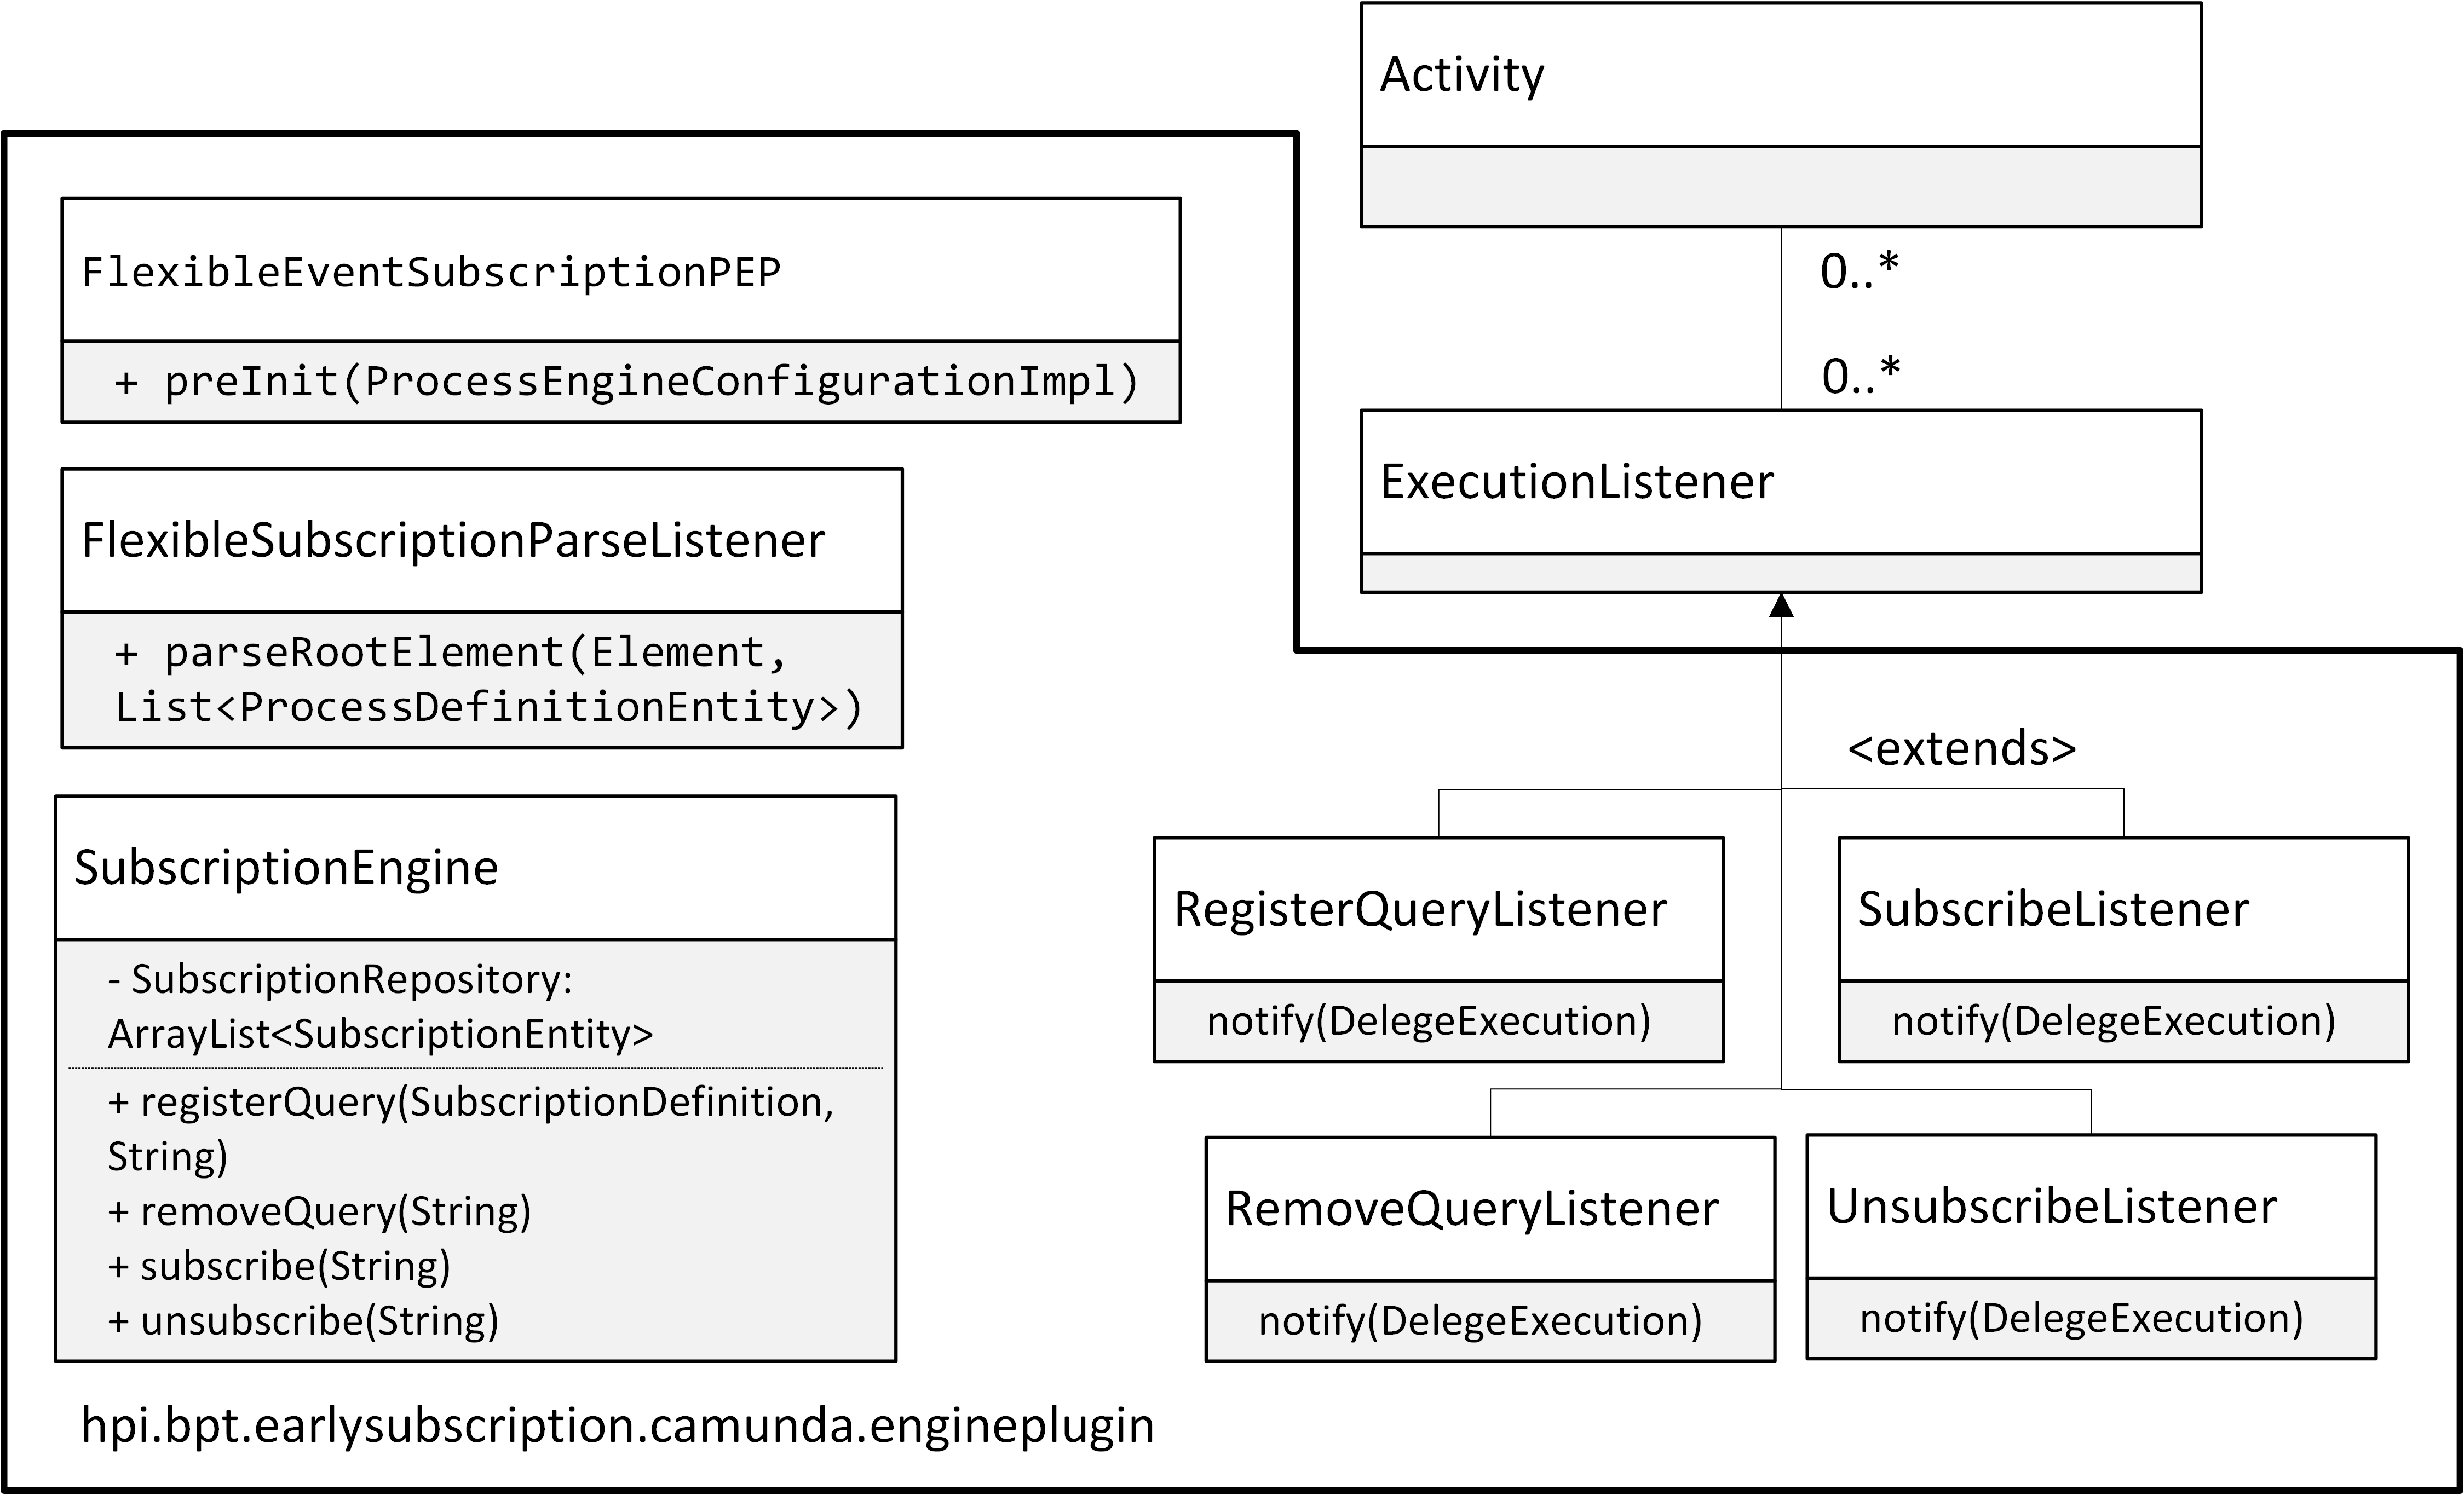
\includegraphics[width=1.0\linewidth]{chapters/implementation/uml-camunda-ext.png}}
	\caption{Excerpt of the UML class diagram of the Camunda Process Engine Plugin}
	\label{fig:camunda-ext-uml}
\end{figure}


% read a model https://docs.camunda.org/manual/7.7/user-guide/model-api/bpmn-model-api/read-a-model/
% bpmn extension elements https://docs.camunda.org/manual/7.7/user-guide/model-api/bpmn-model-api/extension-elements/

\paragraph{SubscriptionEngine}
A new class \textit{SubscriptionEngine} has been introduced, that encapsulates most of the functionality needed to communicate with the API of the event engine.
It offers method representations of all four API-calls, \textit{registerQuery}, \textit{subscribe}, \textit{unsubscribe} and \textit{removeQuery}, translating them into the according HTTP calls which are then executed.
The second, more important functionality is the \textit{SubscriptionRepository}, a list of all available query and subscription identifiers and a mapping to the related process definitions or instances.
As described in \autoref{ch:impl:unicorn-api}, active queries and subscriptions can only be deleted using their unique identifiers. 
When issuing a subscription or registering a query, these identifiers are stored in the repository until the removal call is executed.
Based on the repository information, the SubscriptionEngine can determine the subscription identifiers for provided event element information and execute the remove and unsubscribe operations on the event engine.

\paragraph{ExecutionListeners}
The concept involves four execution listeners, one for each API-call, which are attached to activities through the BPMN parse listener.
Execution listeners can be triggered by the camunda-internal end- or start-event of an activity and can therefor be used to implement the event subscription handling.
Their implementation is concise: each of them is a separate class implementing the \textit{ExecutionListener} interface. They only have one method \textit{notify}, which is called by the engine when the end- or start-event fires.
Within the method, each listener class issues an API-call using the functionality exposed by \textit{SubscriptionManager}.

%\todo[inline]{could mention that registerQuery can be bound either to an instance or to a process definition. this differentiation is made based on the subscriptionDefinition which is passed to the listener on creation.}


\paragraph{Implementation of parseRootElement}
After introducing the \textit{SubscriptionEngine} and the \textit{ExecutionListeners}, this paragraph describes how the listeners are attached to the activities in the course of the execution of \textit{parseRootElement} in our custom \textit{BPMNParseListener}.
By the help of the model representation passed ot the method as an argument of type \textit{Element}, all relevant xml~elements can be extracted based on the element names.
This results in a list of all intermediate and boundary message catch events and receive-tasks and the messages that they reference. The subscription definition is available as a child element of each message.
For each element in the list, the execution now proceeds as outlined in \autoref{ch:extendedprocessengine}.
Depending on the specified subscription time, ExecutionListeners are added at the beginning or end of activity executions or process executions. If the specified subscription time is \textit{Process Deployment}, the provided query is registered immediately using the SubscriptionManager.

This can be exemplified by an intermediate message catch event with subscription time \textit{on process instantiation}:
\begin{itemize}
	\item An instance of \textit{RegisterQueryListener} is added to the start event of the process. The \textit{subscriptiondefinition} is provided to that listener.
	\item The \textit{SubscribeListener} is attached to the start event of the activity representation of the intermediate message event.
	\item To the same activity, objects of \textit{UnsubscribeListener} and \textit{RemoveQueryListener} are registered to be triggered by the end event.
\end{itemize}

\noindent It is worth noting that the available code-base can easily be used to implement the event subscription for message start events, so that processes can be automatically instantiated by events delivered from the event engine.
Considering that process definitions in Camunda are rarely removed completely, the removal of queries on process un-deployment was not implemented. The lack of an obvious intercept point to inject code at that time makes an implementation cumbersome.

\medskip \noindent
Altogether, the enhanced CEP platform and business process engine enable the automatic handling of information provided through the BPMN extension for flexible event subscription.
The event engine exposes functionality for buffered event handling which is accessed through execution listeners during the process execution in Camunda.
The Camunda extension can be flexibly re-used across environments thanks to its implementation in the form of a Process Engine Plugin.
Given these extended features, process designers can conveniently incorporate subscription information for external message events in their executable BPMN models.



